\documentclass{article}
\usepackage[utf8]{inputenc}
\usepackage{pgfplots}
\pgfplotsset{width=10cm,compat=1.9}
\usepackage{amsmath,amssymb,amsthm}
\usepackage{graphicx}
\usepackage{float}
\usepackage{blindtext}
\usepackage{hyperref}
\usepackage{verbatim}
\usepackage{gensymb}
\usepackage{enumerate}
\usepackage{xcolor}
\usepackage{graphicx}
\hypersetup{
    colorlinks=true,
    linkcolor=blue,
    filecolor=magenta,      
    urlcolor=cyan,
    pdftitle={Overleaf Example},
    pdfpagemode=FullScreen,
    }
\usepackage[slovene]{babel}

\setlength{\parindent}{0pt}
\setlength{\parskip}{4pt}

\newcounter{example}[section]
\newenvironment{example}[1][]{\refstepcounter{example}\par\medskip
   \noindent \textbf{Naloga~\theexample. #1} \rmfamily}{\medskip}

\newtheorem*{zgled}{Zgled}

\title{Geometrija}
\author{Bor Bregant}
\date{\vspace{-5ex}}

\begin{document}

\maketitle

\section{Trikotnik}

Višina trikotnika je daljica, pravokotna na stranico... Višinska točka (ortocenter).

Težiščnica trikotnika je daljica, ki povezuje oglišče in razpolovišče stranice. Težišče trikotnika razdeli težiščnice $1:2$.

...

\section{Krog in krožnica}

Krožnica je množica točk v ravnini, ki so enako oddaljene (za polmer) od fiksne točke, ki jo imenujemo središče.  $K = \{T;\ d(T,S)=r\}$. Krog podobno, le $\leq$.

Tangenta ali dotikalnica je premica, ki ima s krožnico eno samo skupno točko in je pravokotna na radij.

Sekanta je premica, ki ima s krožnico dve skupni točki. Tetiva je daljica, ki povezuje dve točki na krožnici. Lok

Skupna slika vsega zgoraj

Središčni kot je kot, ki ima vrh v središču kroga, kraka pa potekata skozi dve točki na krožnici. Obodni kot nad lokom $AB$. Središčni kot je še enkrat večji od obodnega kota nad istim lokom z dokazom.\\
\begin{figure}[H]
    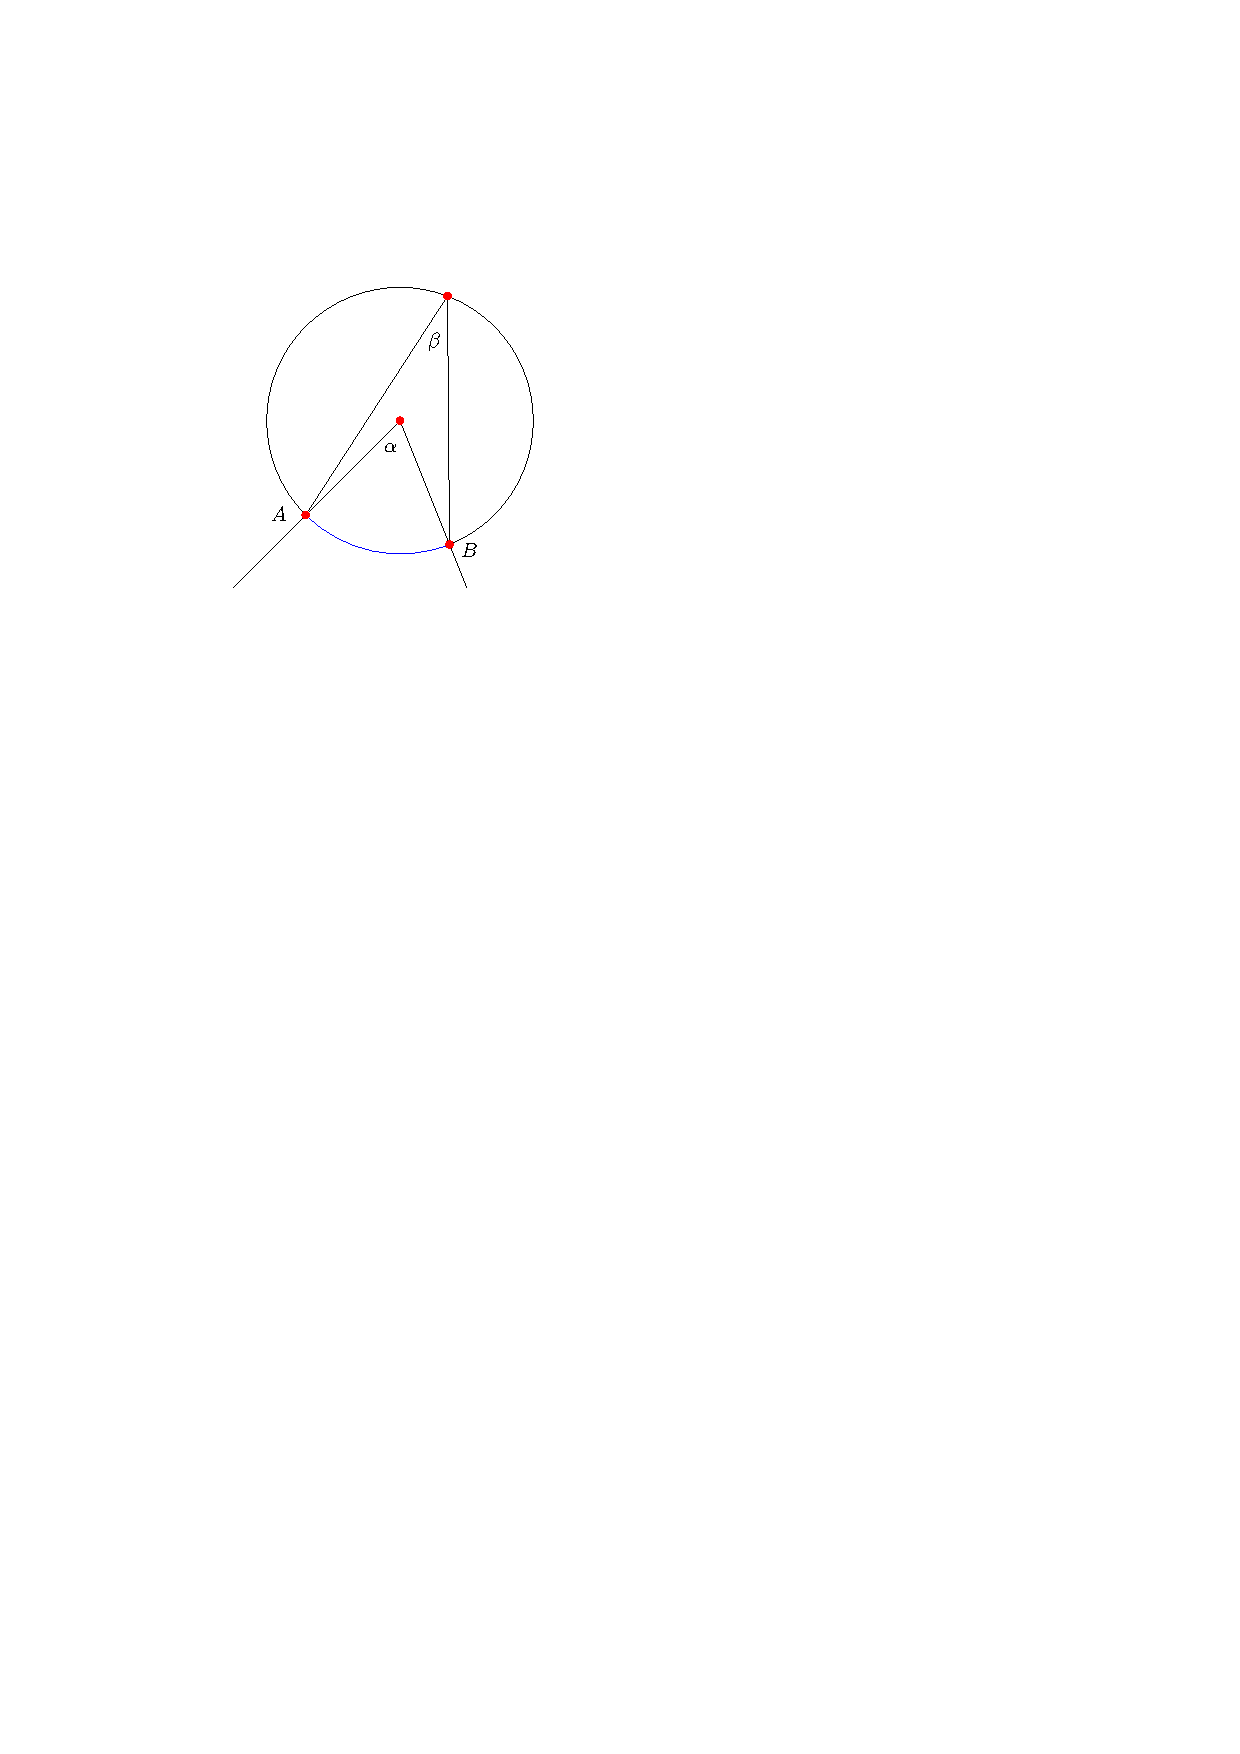
\includegraphics[width=0.4\textwidth]{srediscni_kot.pdf}
    \centering
\end{figure}
Posledica: Vsi obodni koti nad istim lokom so skladni.\\
Posledica: Če je središčni kot iztegnjeni kot, je njegov obodni kot pravi kot (Talesov izrek).


Risanje tangente na krožnico skozi poljubno točko s pomočjo Talesovega izreka
\begin{enumerate}[i]
    \item Poveži $S$ (središče) in $T$ (zunanja točka).
    \item Razpolovišče $ST\rightarrow S'$
    \item Polkrog iz $S'$, radij $|SS'|$
    \item Dobimo dve tangenti
\end{enumerate}
\begin{figure}[H]
    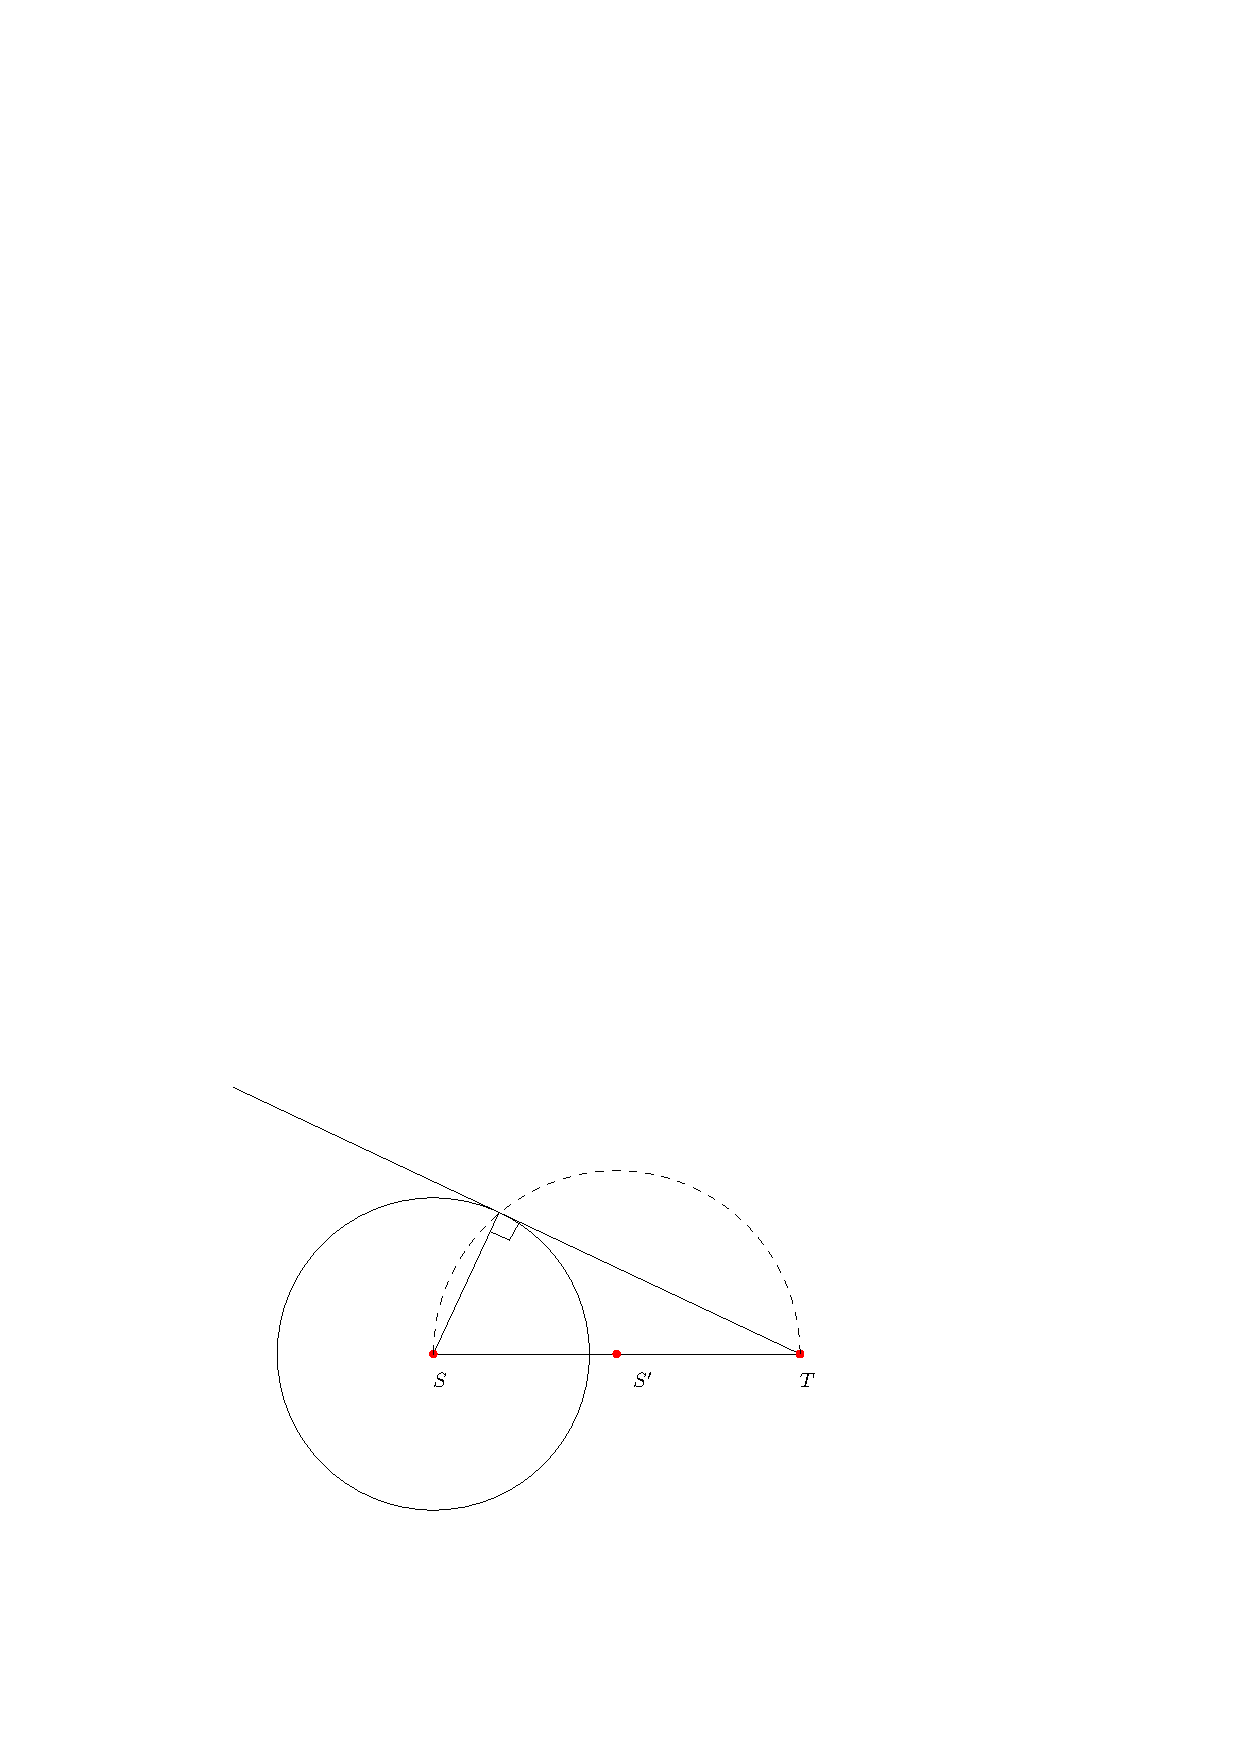
\includegraphics[width=0.6\textwidth]{risanje_tangente.pdf}
    \centering
\end{figure}

Merjenje kotov:

Stopinje, minute, sekunde\\
$1\degree$ je $\frac{1}{360}$ polnega kota\\
$1\degree=60'$ in $1'=60''$.

Radiani:\\
Kot meri en radian, če mu priprada lok z dolžino radija
\begin{figure}[H]
    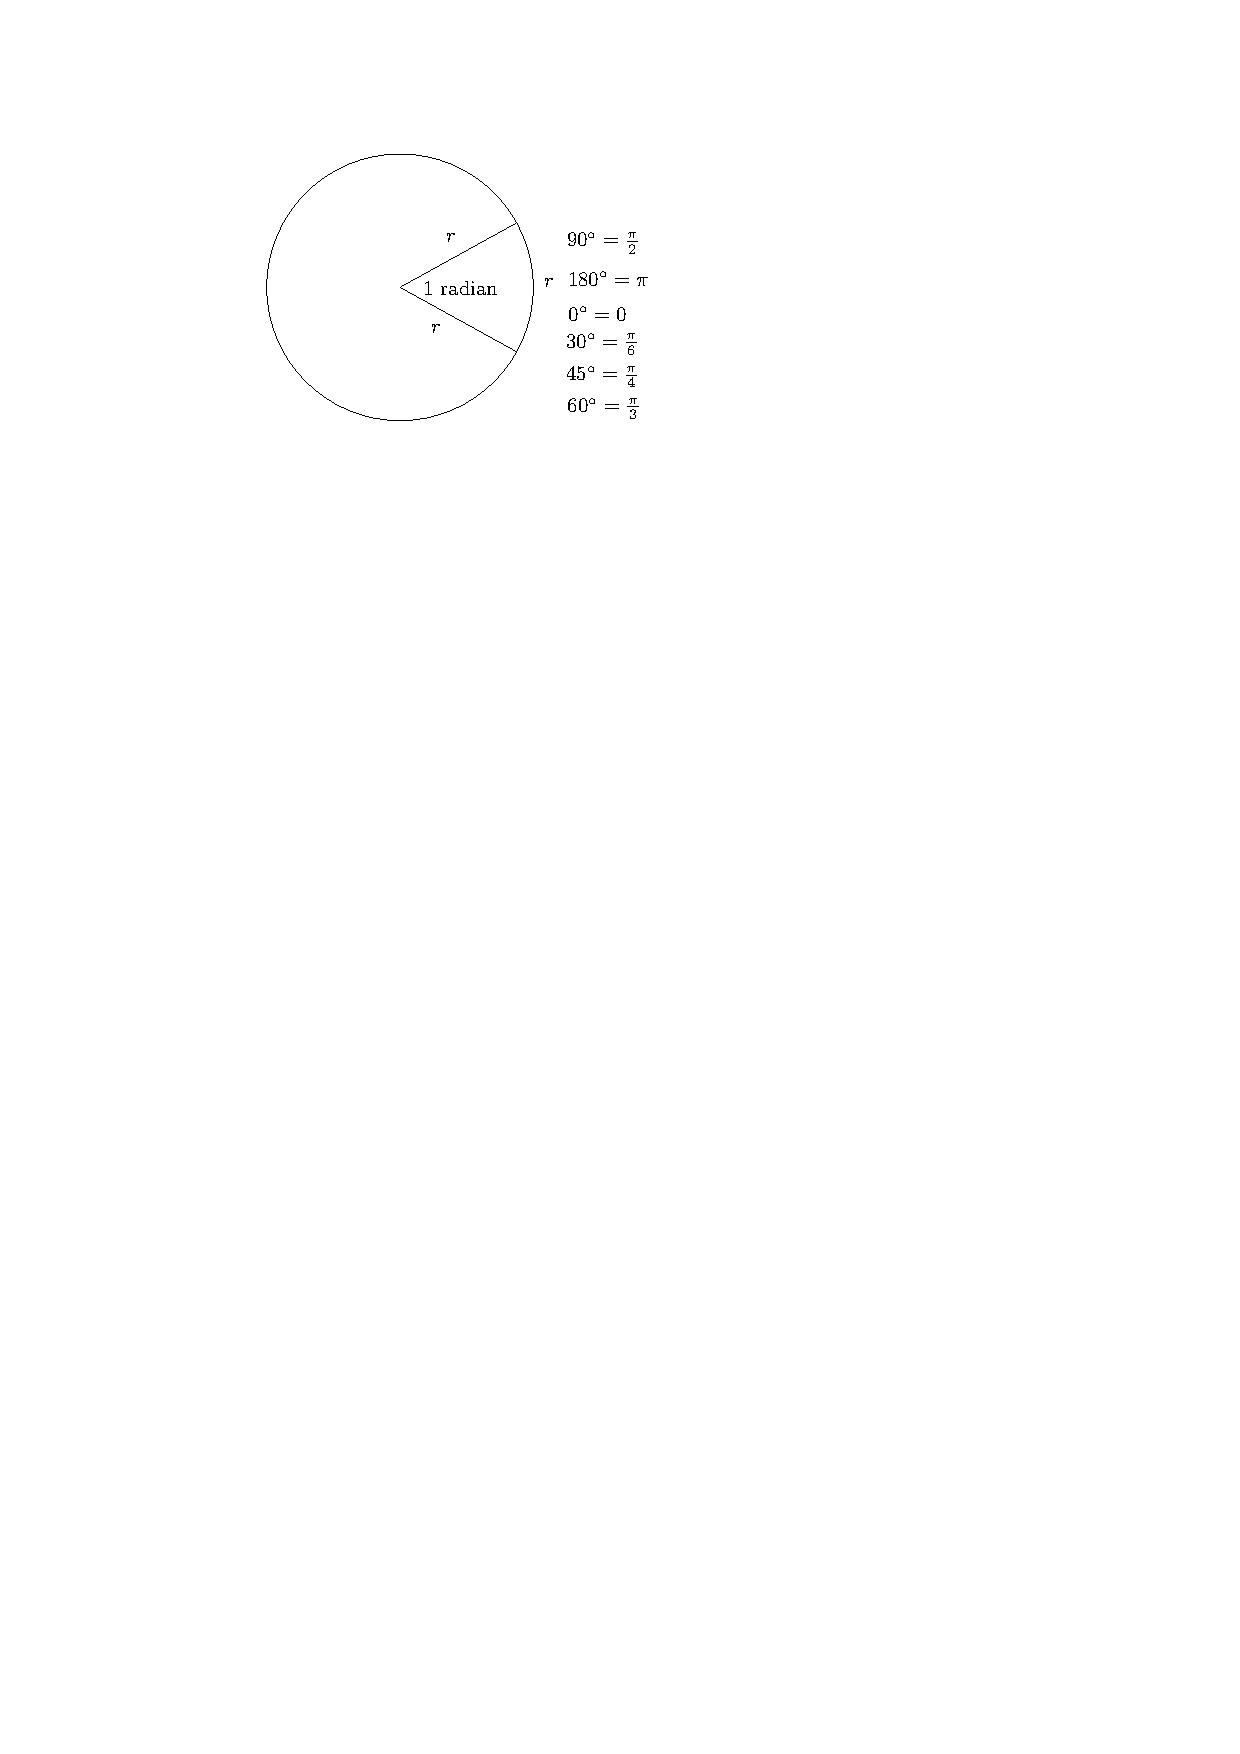
\includegraphics[width=0.6\textwidth]{radiani.pdf}
    \centering
\end{figure}
Polni kot: $2\pi$ radianov\\


\begin{zgled}
    Nariši $\Delta ABC$, v katerem $c=6cm,\ v_c = 2cm,\ \gamma=60\degree$.\\
    \textcolor{gray}{Ideja: Začnemo s $c$ in naredimo vzporednico za višino. Želimo središčni kot $120\degree$. Ker je središčni enakokrak, bosta ostala kota $30\degree$. $\gamma$ bo torej obodni kot za krožnico s središčem $S$ in polmerom $AS$.}
\end{zgled}

\begin{example}
    Konstruiraj trikotnik s podatki $a=5cm,\ t_a =4cm,\ \alpha=30\degree$.
\end{example}








\section{Štirikotnik in pravilni $n$-kotnik}

Vsota notranjih kotov štirikotnika je $360\degree$. \textit{dokaz s triangulacijo}

\subsection*{Paralelogram}

\begin{figure}[H]
    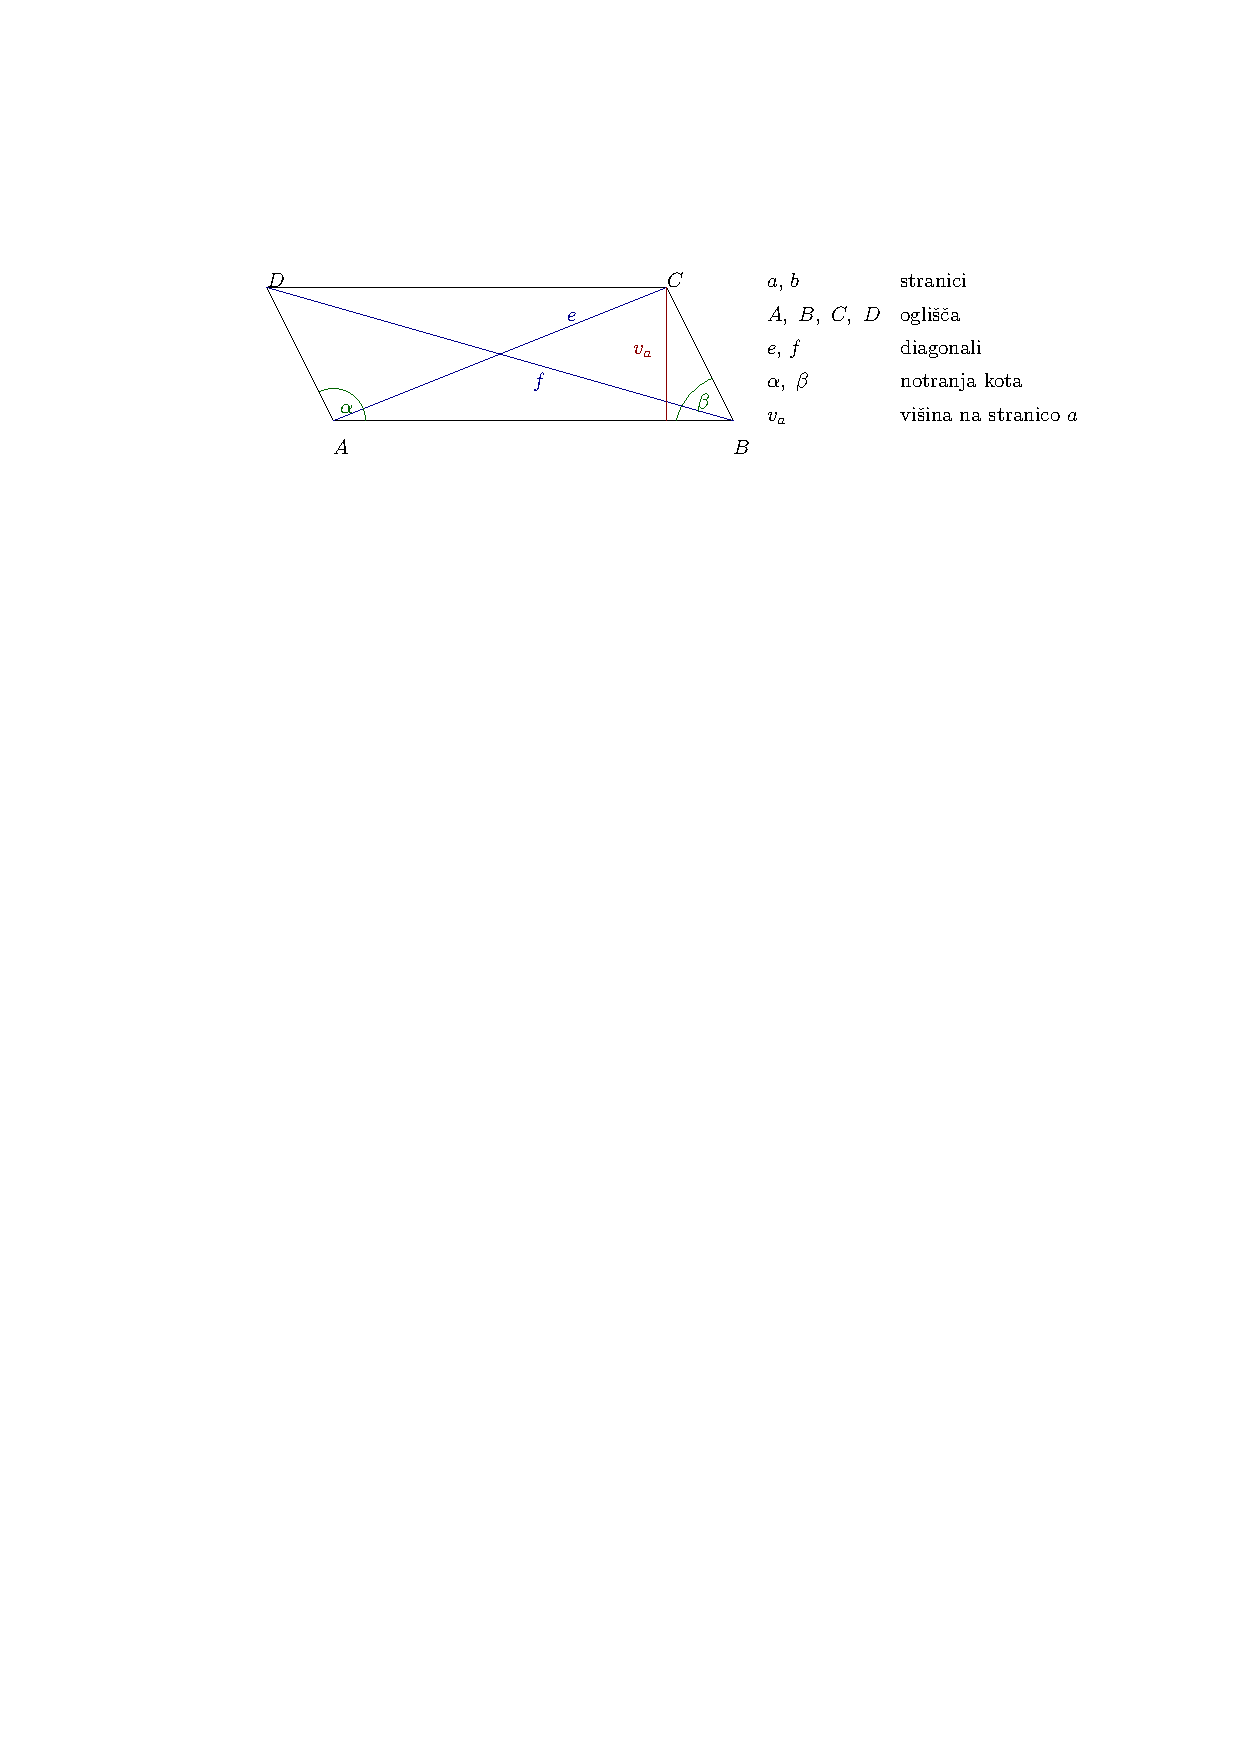
\includegraphics[width=1\textwidth]{paralelogram.pdf}
    \centering
\end{figure}

\begin{enumerate}[i]
    \item Dva para vzporednih stranic
    \item Diagonali se razpolavljata
    \item Poljubna sosednja kota sta suplementarna
    \item Poljubna nasprotna kota sta enako velika
  \end{enumerate}


Pravokotnik = pravokotni paralelogram

Romb = enakostranični paralelogram (diagonali se razpolavljata pod pravim kotom)

Kvadrat = enakostranični pravokotnik

Trapez = štirikotnik, ki ima par vzporednih stranic ($\alpha$ in $\delta$ suplementarna) (enakokraki trapez)

Srednjica trapeza (povezuje razpolovišči krakov in je vzporedna osnovnicama) ima dolžino $s=\frac{a+c}{2}$

Deltoid = štirikotnik, ki ima dva para sosednjih enako dolgih stranic (diagonali sta pravokotni, ena se z drugo razpolavlja \& dva notranja kota sta skladna).

\begin{figure}[H]
    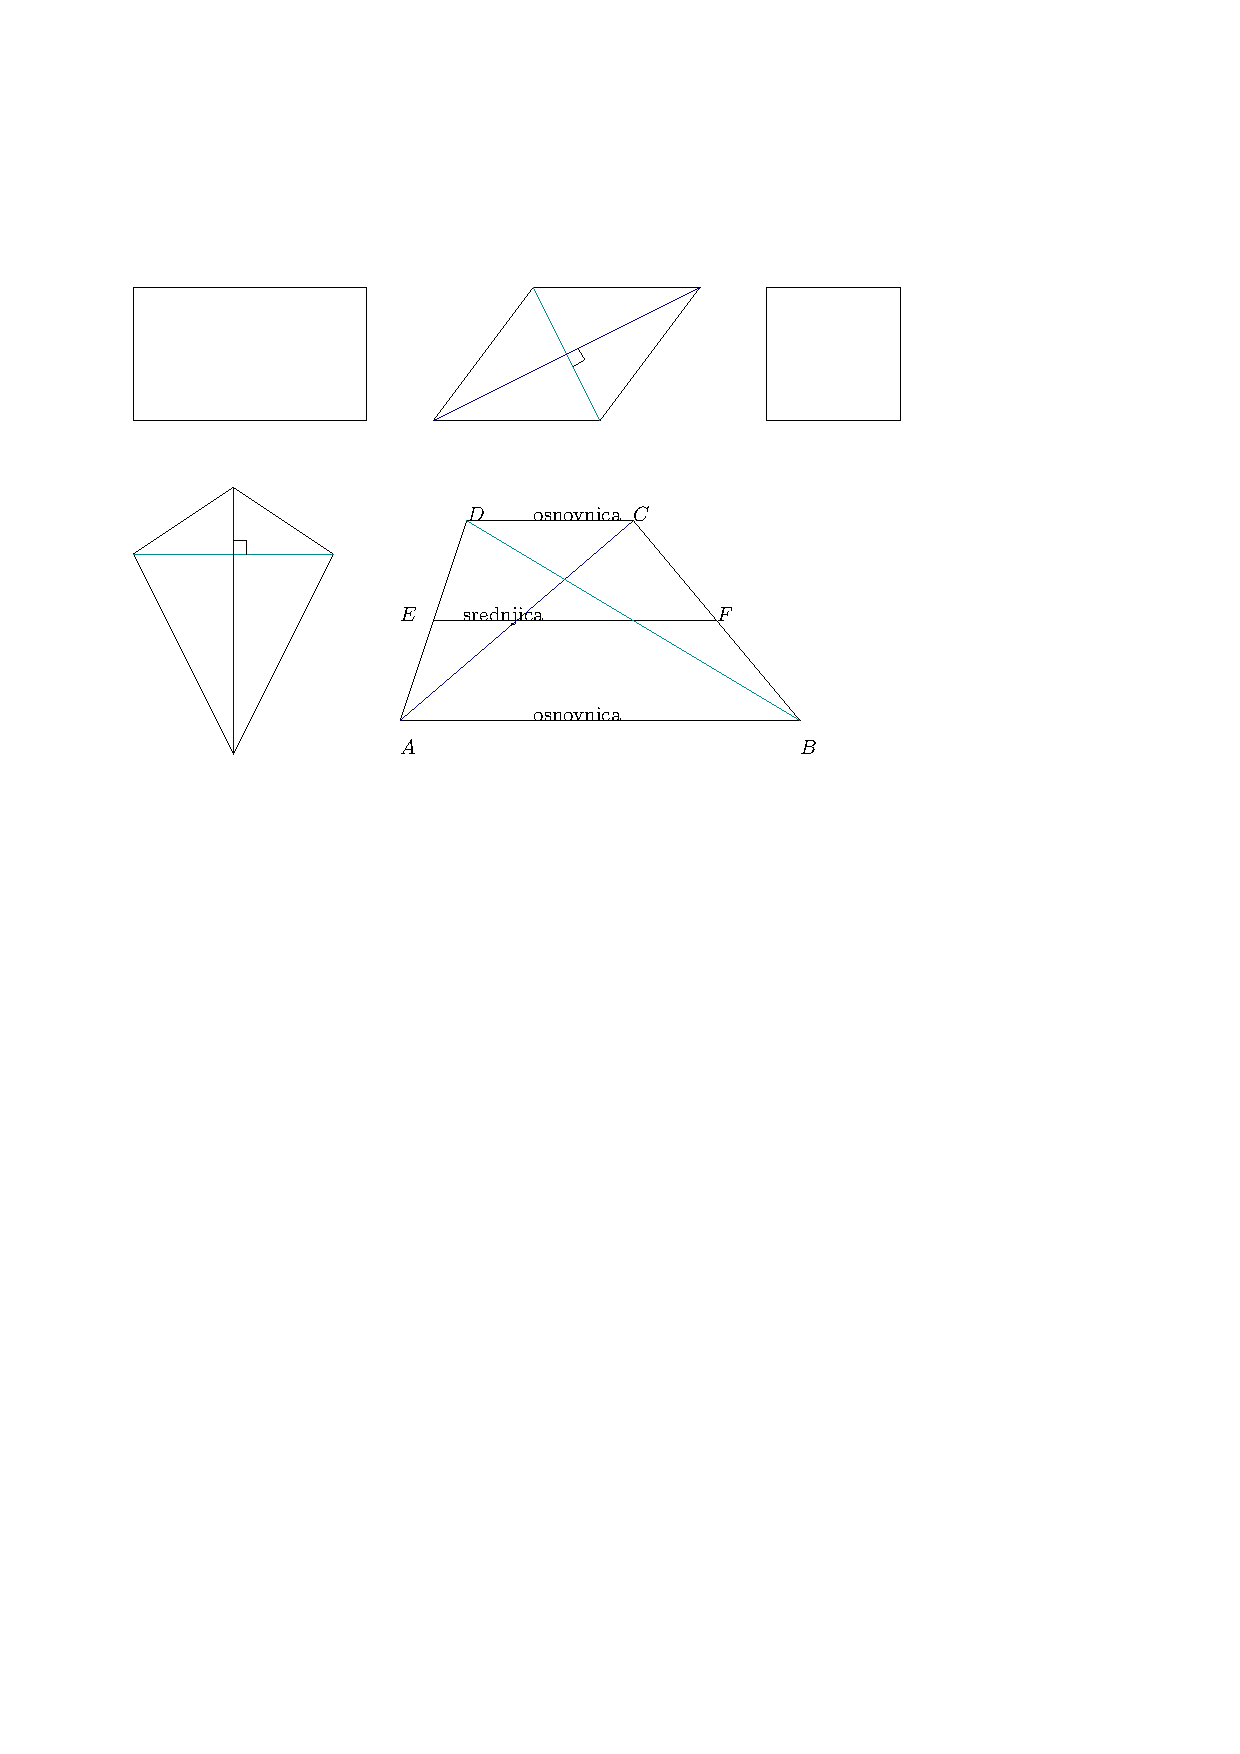
\includegraphics[width=1\textwidth]{liki.pdf}
    \centering
\end{figure}

\begin{zgled}
    Nariši paralelogram $ABCD$, za katerega velja $\alpha=120\degree,\ e=2.5cm,\ v_a=2cm$.
\end{zgled}

\begin{zgled}
    Nariši romb $ABCD$, katerega diagonali merita $e=5cm$ in $f=4cm$.
\end{zgled}

\begin{zgled}
    Nariši pravokotnik $ABCD$, za katerega velja $a=4cm$ in $f=6cm$.
\end{zgled}

\begin{zgled}
    Nariši trapez $ABCD$, za katerega velja $a=4.5cm$, $\beta=45\degree$, $e=3.3cm$ in $f=5cm$.
\end{zgled}

\begin{zgled}
    Nariši trapez $ABCD$, za katerega velja $\alpha=60\degree$, $d=3cm$, $c=2cm$ in $f=6cm$.
\end{zgled}

\begin{zgled}
    Nariši deltoid $ABCD$, za katerega velja $e=4cm$, $f=7cm$ in $a=5cm$.
\end{zgled}

\begin{zgled}
    S pomočjo paralelograma na sliki nariši trikotnik $ABC$, kjer $b=4cm$, $t_a =4.5cm$ in $\alpha=75\degree$.
\end{zgled}

\begin{example}
    DN 119, 121b, 128acd, 132a, 133ac
\end{example}


Tangentni štirikotnik (očrtamo krožnico, $a+c=b+d$ z dokazom)

Tetivni štirikotnik (včrtamo krožnico, $\alpha+\gamma=\beta+\delta=180\degree$ z dokazom)

Pravilni $n$-kotnik - vse stranice in notranji koti enaki. Vsota kotov = $(n-2)180\degree$. 

\begin{figure}[H]
    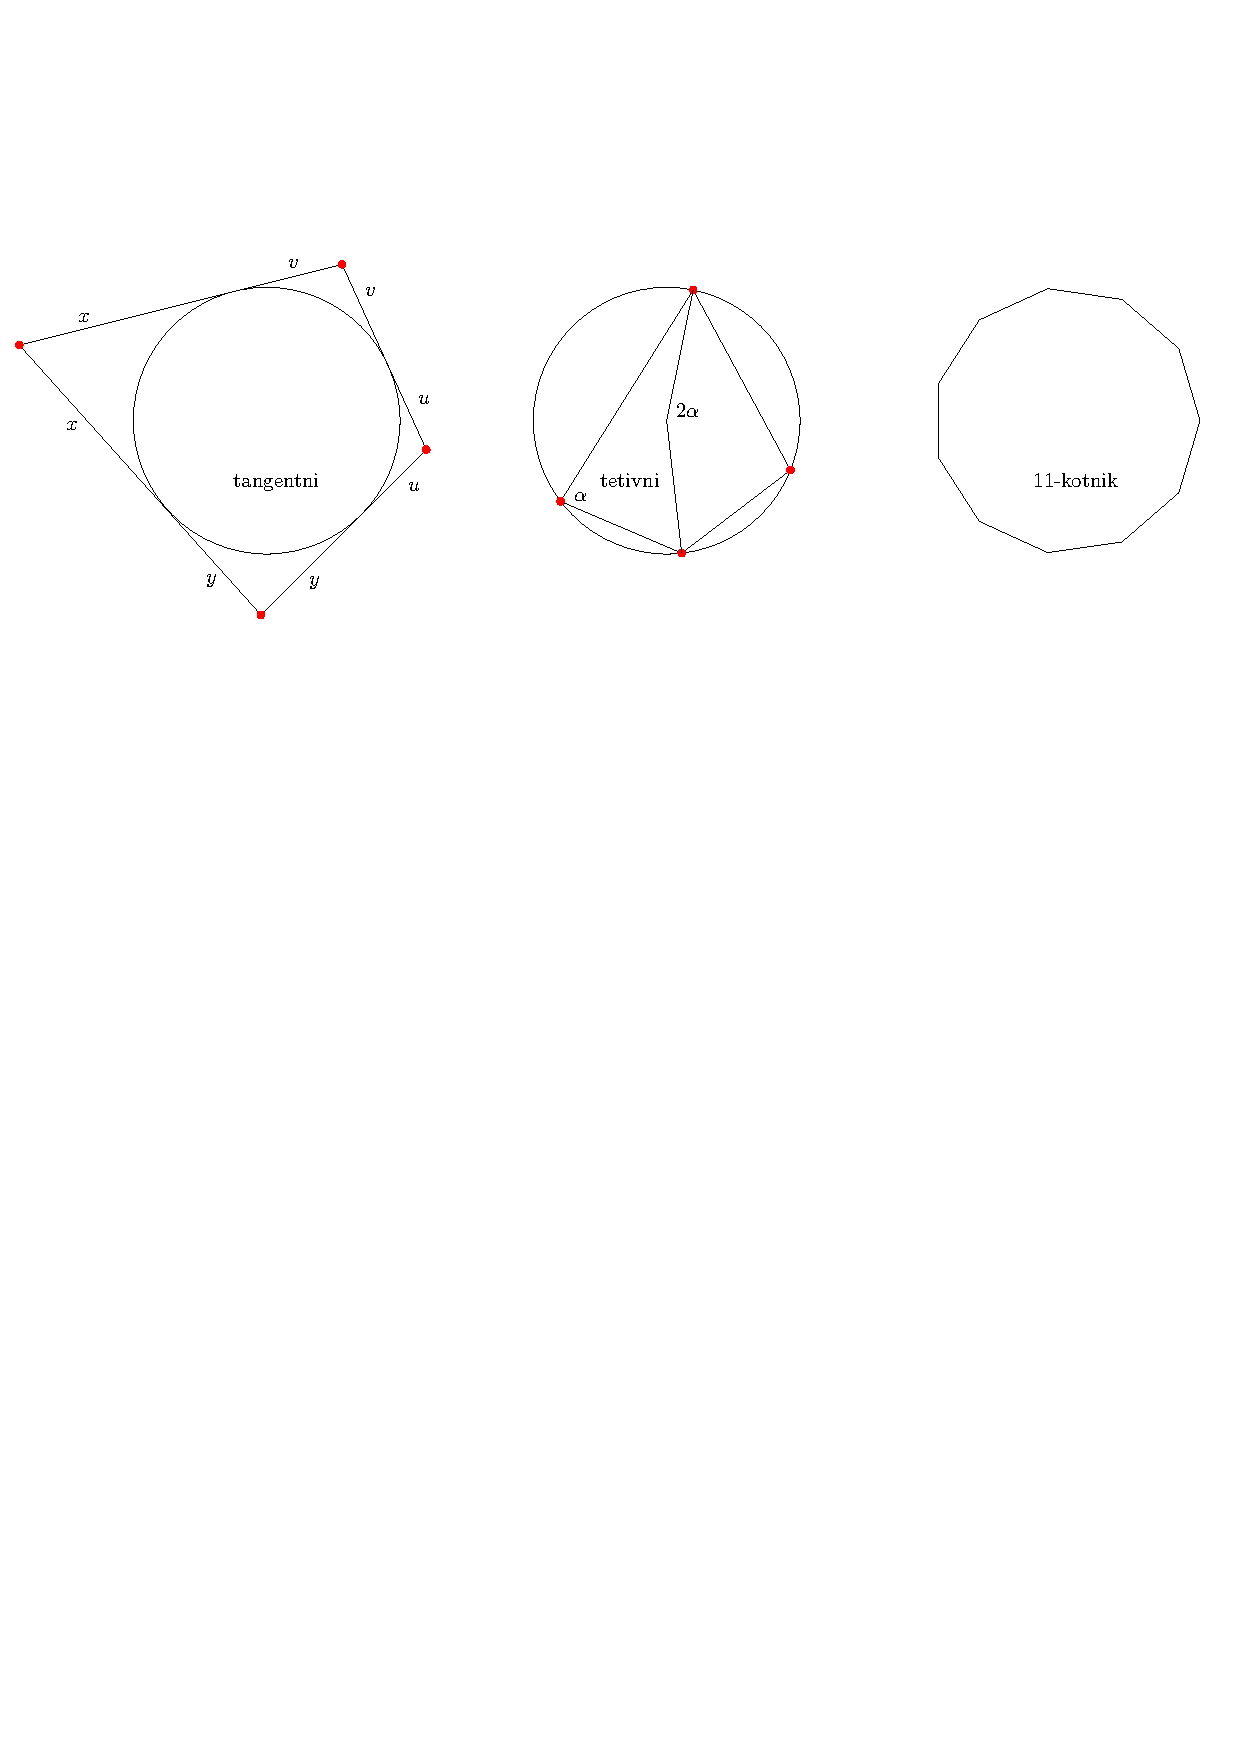
\includegraphics[width=1\textwidth]{liki_2.pdf}
    \centering
\end{figure}

\begin{zgled}
    Glede na sliko določi \textcolor{gray}{$|XY|$} in $\angle XYZ$.
    \begin{figure}[H]
    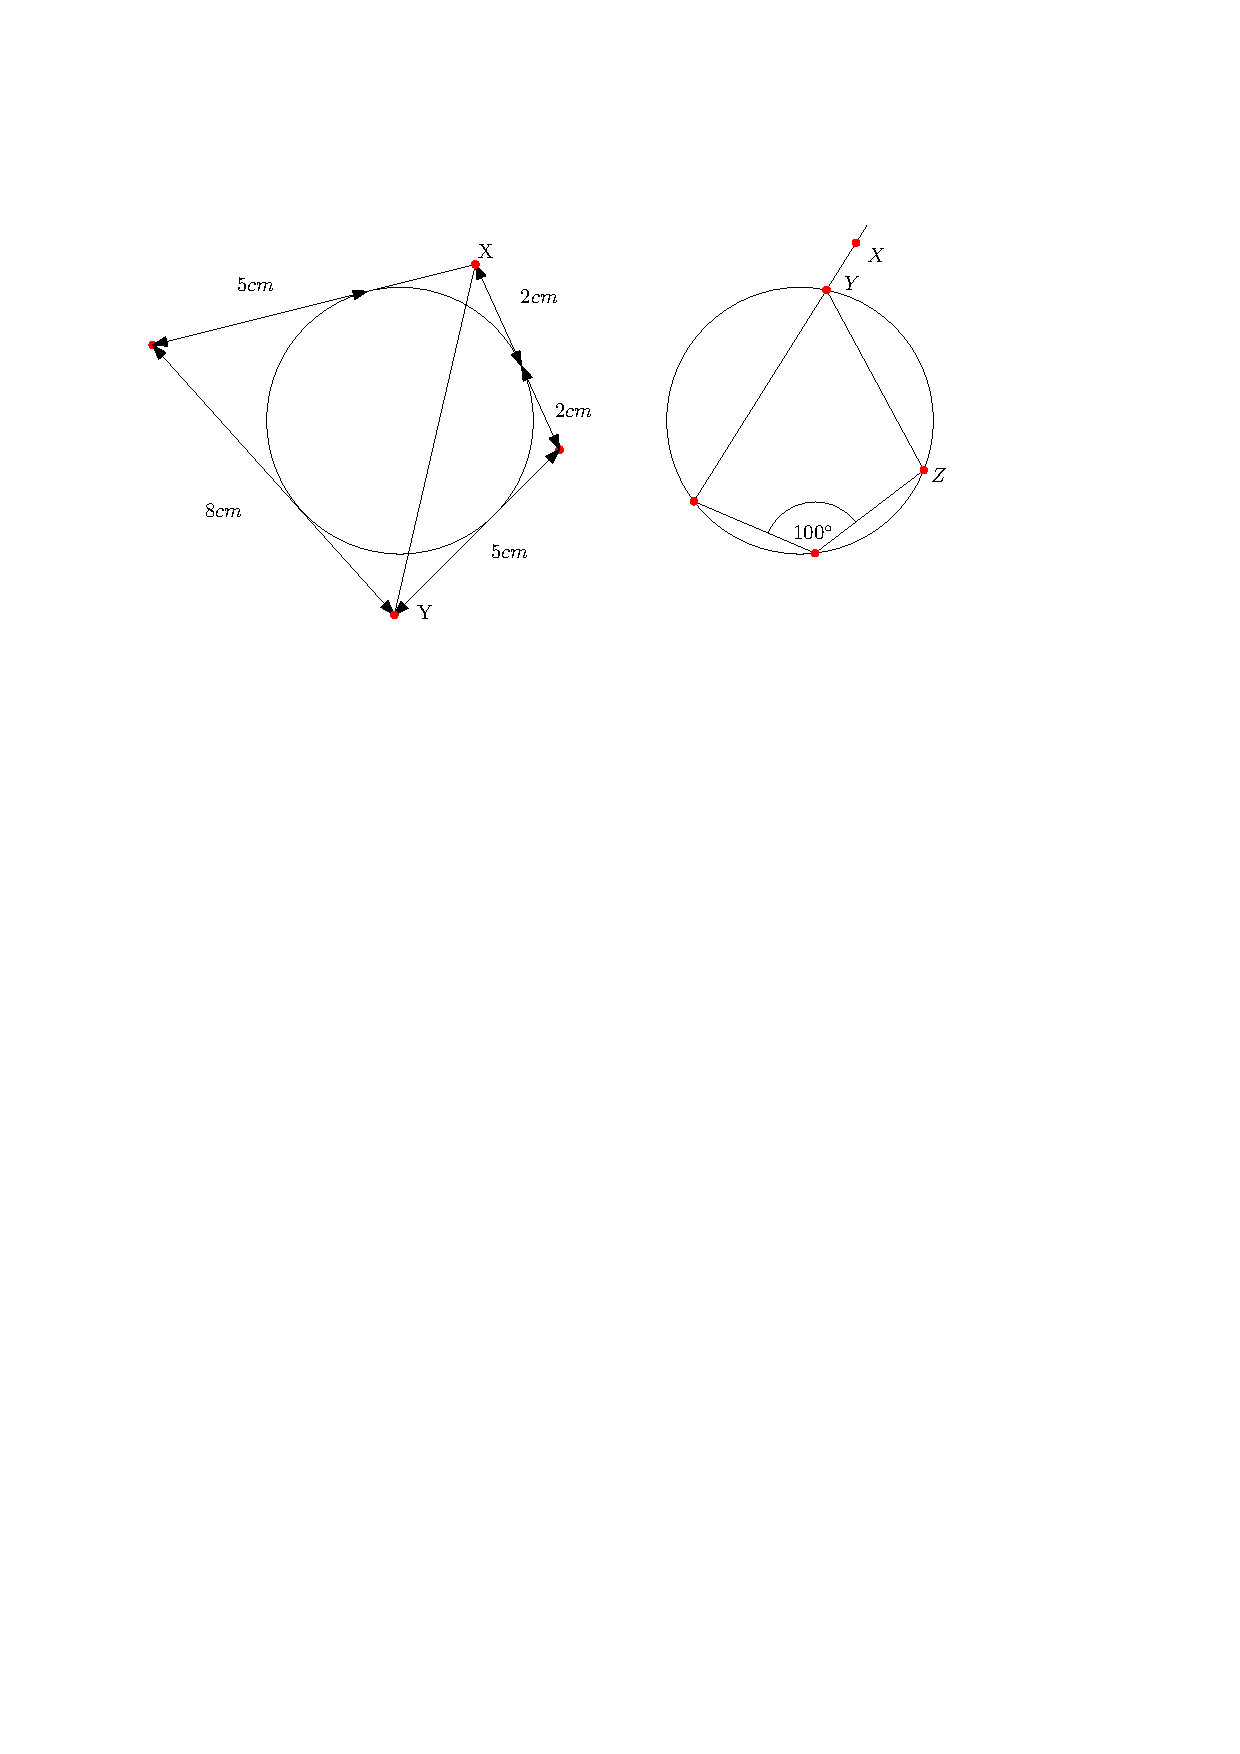
\includegraphics[width=0.8\textwidth]{naloga.pdf}
    \centering
    \end{figure}
\end{zgled}

\begin{zgled}
    Načrtaj tangenten trapez s podatki $a=6cm$, $\alpha =60\degree$ in polmerom včrtane krožnice $r=2cm$.\\
    \textcolor{gray}{$a, \ \alpha \rightarrow$ simetrala $\alpha$, vzporednica $a$ oddaljena za $r$, $\rightarrow$ $S$}
\end{zgled}

\begin{zgled}
    Če $n$-kotniku podvojimo število stranic, se njegovo število diagonal pomnoži z $5$. Kateri $n$-kotnik je to.
\end{zgled}

\begin{example}
    Kateri $n$ kotnik ima $3$ diagonale več kot stranic?
\end{example}


\section{Podobnost}

\begin{zgled}
    Daljici $AB$ in $CD$ sta v razmerju $5:4$, vsota njunih dolžin pa je $63cm$. Izračunaj dolžini $AB$ in $CD$.
\end{zgled}

\begin{zgled}
    Daljico $AC$ razdeli na dva dela, da bo veljalo $|AB|:|BC|=3:4$, kjer $|AC|=5cm$.
\end{zgled}

Trikotnika $ABC$ in $A_1 B_1 C_1$ sta podobna, če imata enaka razmerja vseh stranic in enake vse notranje kote ali ekvivalentno če se ujemata v:
\begin{enumerate}[i]
    \item razmerju dveh enakoležnih stranic $a:a_1 = b:b_1 =c: c_1$.
    \item dveh notranjih kotih npr. $\alpha = \alpha_1$, $\beta =\beta_1$.
    \item razmerju dveh stranic in vmesni kot npr. $\alpha =\alpha_1$, $b:b_1 = c: c_1$.
    \item razmerju dveh stranic in v kotu nasproti daljše stranice.
  \end{enumerate}

  Relacija podobnosti je ekvivalenčna:
  \begin{enumerate}[i]
    \item Refleksivnost $L\sim L$
    \item Simetričnost $L_2\sim L_1 \Rightarrow L_1 \sim L_2$
    \item Tranzitivnost $L_1 \sim L_2 \land L_2 \sim L_3 \Rightarrow L_1 \sim L_3$.
  \end{enumerate}

  Središčni razteg (homotetija) s središčem v točki $O$ in faktorjem $k$ je preslikava, ki daljico $OA$ preslika v daljico $OA'$, da velja $|OA'|=k\cdot |OA|$.
  \begin{enumerate}[i]
    \item Ohranja kote (oblike, tudi vzporednost)
    \item $|k|>1$ pomeni razteg, $|k|<1$ pomeni skrčitev, $k<0$ doda še zrcaljenje.
    \item Podobnostna preslikava, saj like slika v njim podobne like.
  \end{enumerate}
  \begin{figure}[H]
    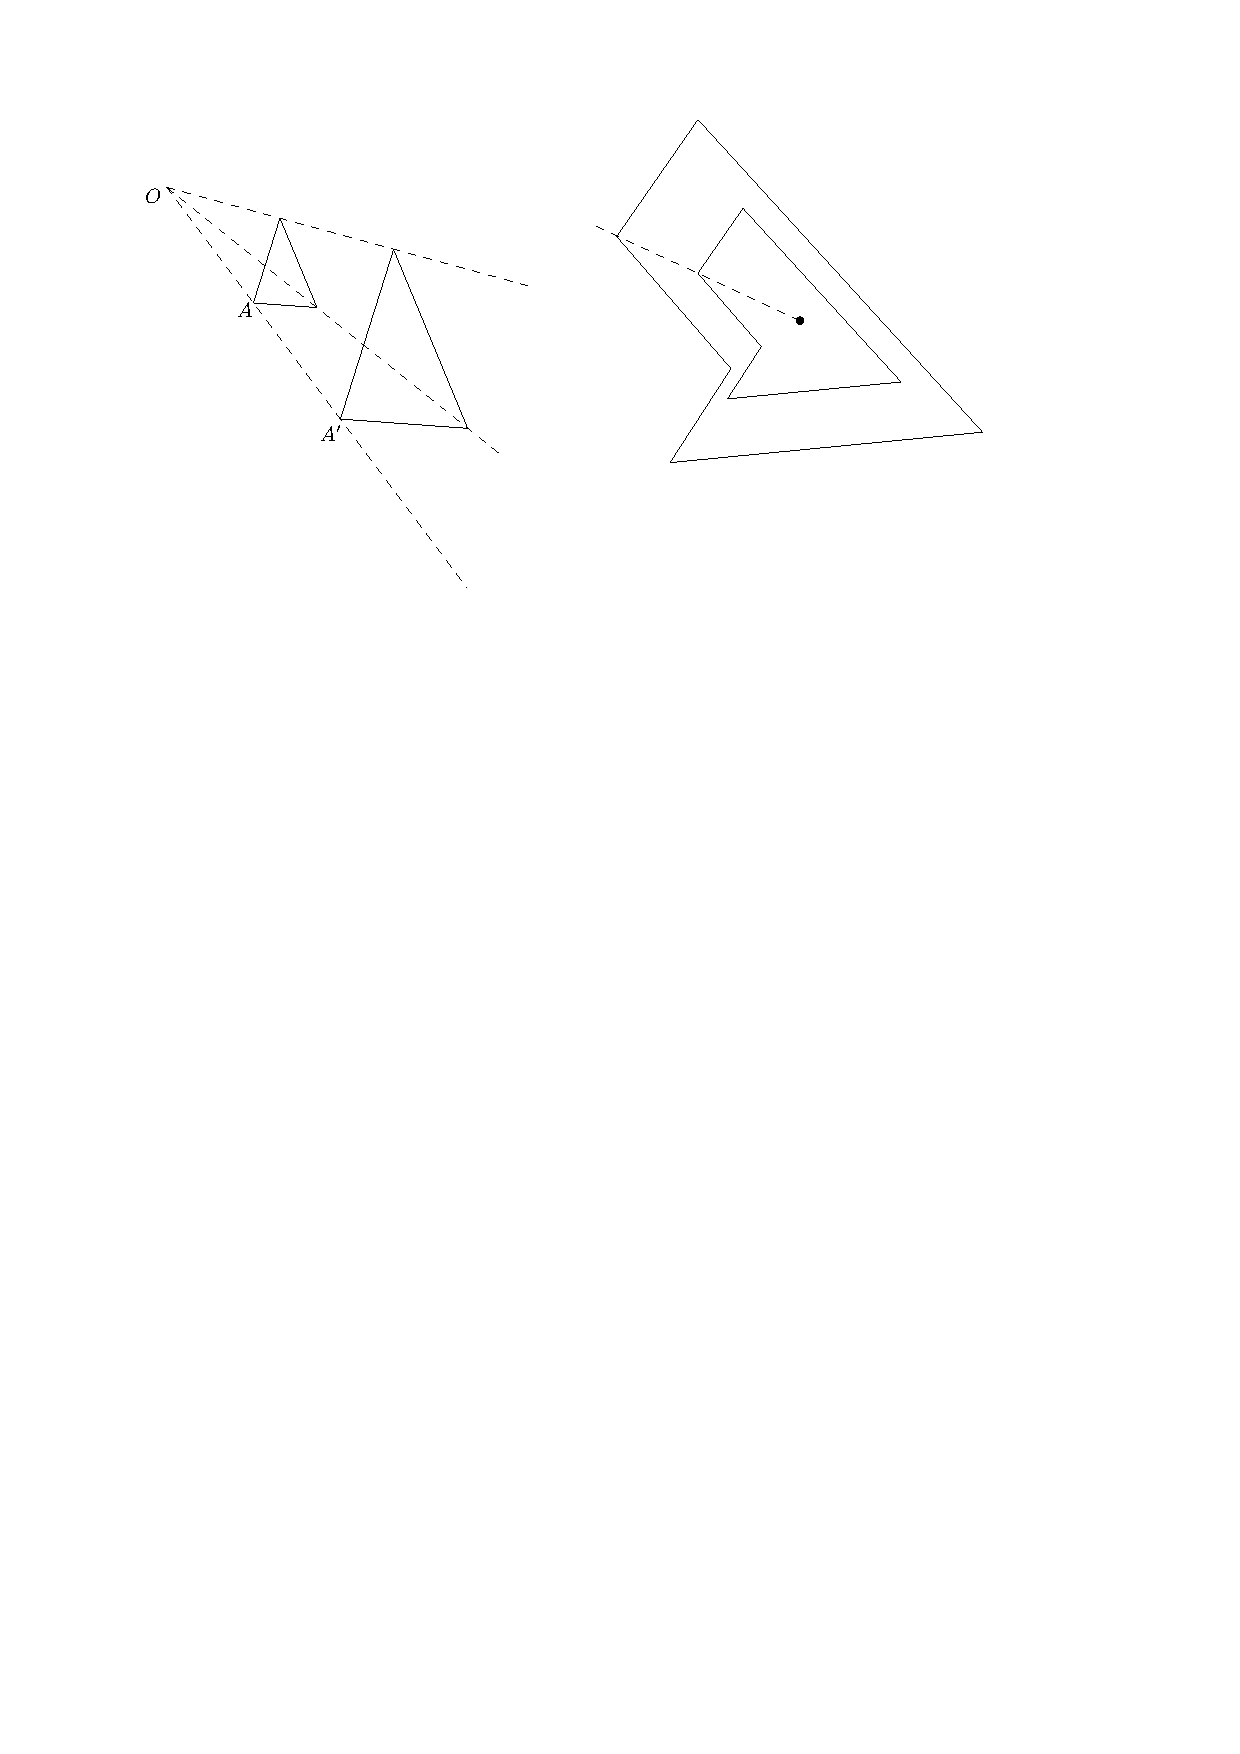
\includegraphics[width=0.65\textwidth]{homotetija.pdf}
    \centering
    \end{figure}

  Geometrijska sredina $a:x=x:b\rightarrow x=\sqrt{ab}$\\
  Primer: Geometrijska sredina $2$ in $18$ je $6$. Velja $2\times 18$ = $6\times 6$ (ploščina)\\
  Primer kasneje: Višinski izrek

  Razmerje = kvocient dveh količin (npr. dolžin daljic)\\
  Sorazmerje = enakost dveh razmerij\\
  Talesov izrek:
\begin{figure}[H]
    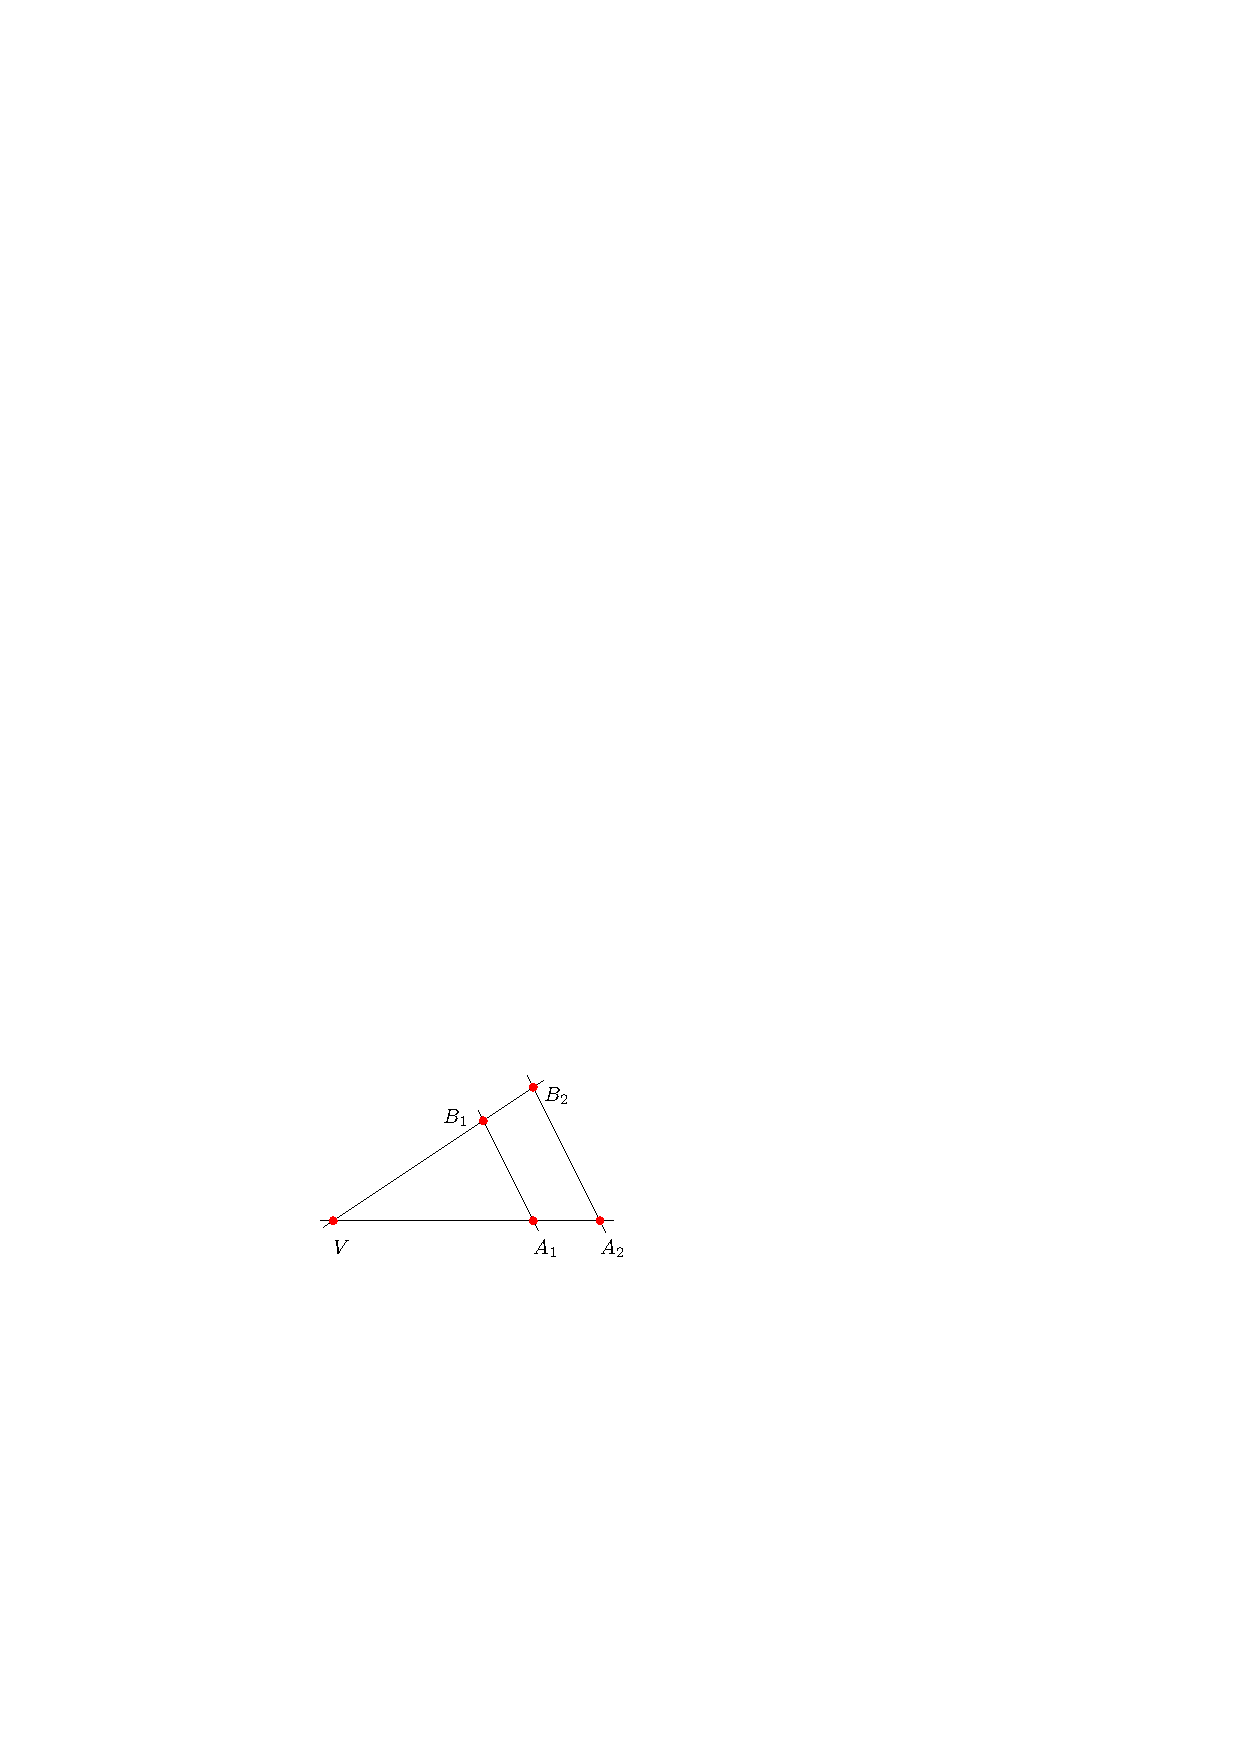
\includegraphics[width=0.6\textwidth]{tales_sorazmerja.pdf}
    \centering
\end{figure}

\begin{zgled}
    Stranice $\Delta ABC$ so v razmerju $2:5:4$, njegov obseg pa meri $5.5cm$. Kako dolge so stranice trikotnika.
\end{zgled}

\begin{zgled}
    V $\Delta ABC$ narišemo daljico $BD$ tako, da točka $D$ razdeli stranico $AC$ na odseka $|AD|=7cm$ in $|DC|=9cm$, ter da je $\angle BDC$ = $\angle ABC$. Izračunaj $|BC|$ in $|BD|:|AB|$.
\end{zgled}


\begin{zgled}
    V trapezu $ABCD$ sta kota $\angle ADC$ in $\angle ACB$ skladna. Izračunaj $|AC|$, če je $|AB|=27cm$ in $|DC|=12cm$.
\end{zgled}

\begin{example}
    DN 143ac, 145abc, 148
\end{example}

Višinski izrek $v^2 =a_1 b_1$, Evklidov izrek $a^2=a_1 c$, $b^2=b_1 c$, Pitagorov izrek $c^2=a^2+b^2$.
    \begin{figure}[H]
    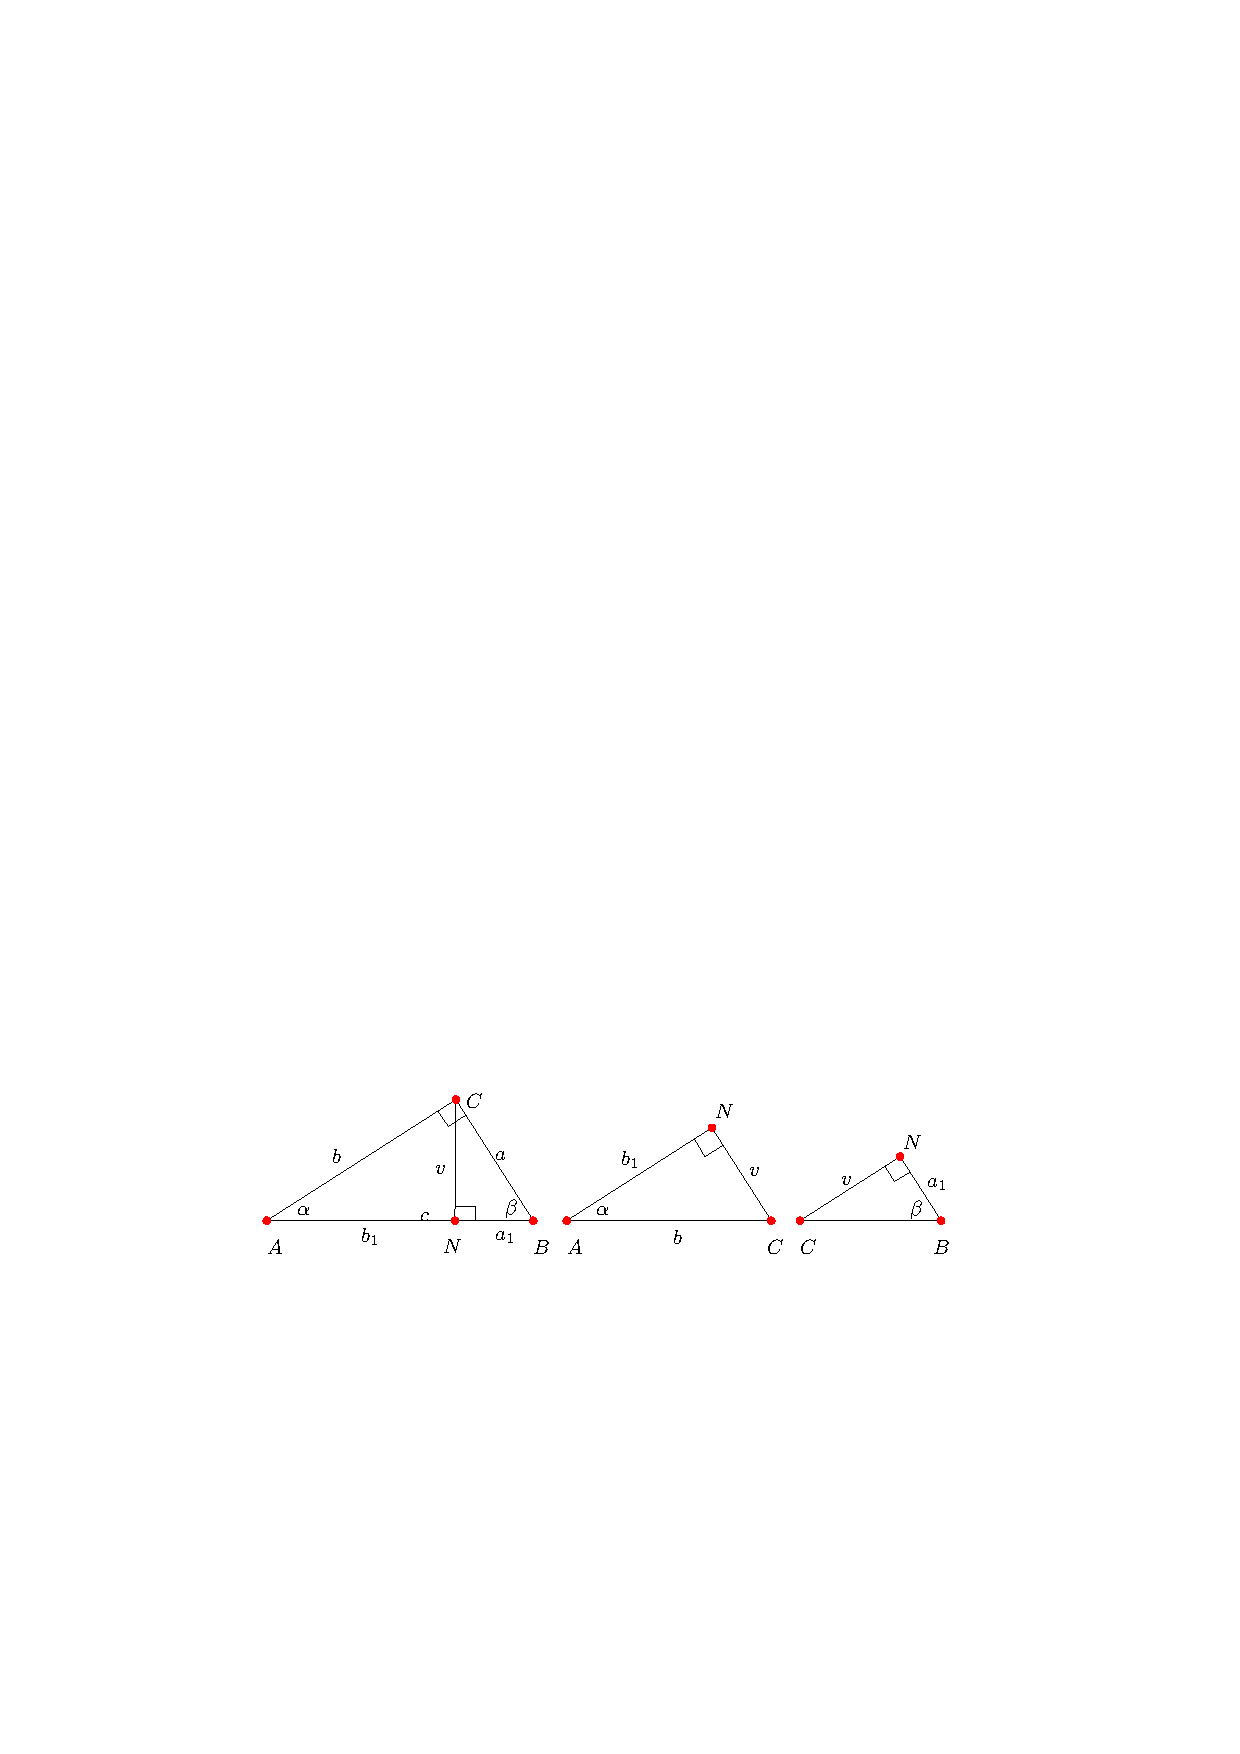
\includegraphics[width=0.6\textwidth]{evklidov_visinski.pdf}
    \centering
    \end{figure}

Višinski $v:b_1=a_1:v$\\
Evklidov $a:c=a_1:a$ in podobno za $b$\\
Pitagorov $a^2+b^2=a_1 c+b_1 c = (a_1 +b_1) c=c^2$.



\begin{zgled}
    Narišimo daljico dolžine $\sqrt{15}$.
\end{zgled}

\begin{zgled}
    V pravokotnem trikotniku izračunaj pravokotno projekcijo katete $b$ na hipotenuzo, če je $b=7cm$ in $a=4cm$.
\end{zgled}

\begin{zgled}
    Izračunaj dolžini višine na hipotenuzo in projekcije neznane katete na hipotenuzo v pravokotnem trikotniku $ABC$, pri katerem je $c=9cm$ in $b=5cm$.
\end{zgled}

\begin{zgled}
    Izračunaj velikost diagonale kvadrata in višine enakostraničnega trikotnika, če je obakrat stranica enaka $a$.
\end{zgled}

\begin{zgled}
    Dve ladji sta ob isti uri izpluli iz pristanišča, ena proti vzhodu, druga proti jugu. Po nekaj urah sta bili $17$ milj narazen. Pri tem je ladja proti jugu naredila $7$ milj več kot ladja, ki pluje proti vzhodu. Kolikšno pot sta prevozili.
\end{zgled}
    
\begin{zgled}
    Nariši $\Delta ABC$, kjer $a:b=3:4$, $\gamma =60\degree$ in $t_c = 2cm$.
\end{zgled}

\begin{example}
    DN 149, 153, 164aceg, 167, 172
\end{example}

\end{document}